\section{Fluxo de avaliação de vida à fadiga em dutos em vão livre}\label{chap:workflow}


Baseado nos estudos e \textit{oficinas} realizados para o desenvolvimento deste trabalho. Pôde-se estabelecer que a análise de vida a fadiga em dutos em vão livre compreende o fluxograma apresentado na \autoref{fig:fluxograma}.

\begin{figure}[!ht]
    \centering
    \caption{Fluxo de avaliação de vida à fadiga em dutos em vão livre.}\label{fig:fluxograma}
    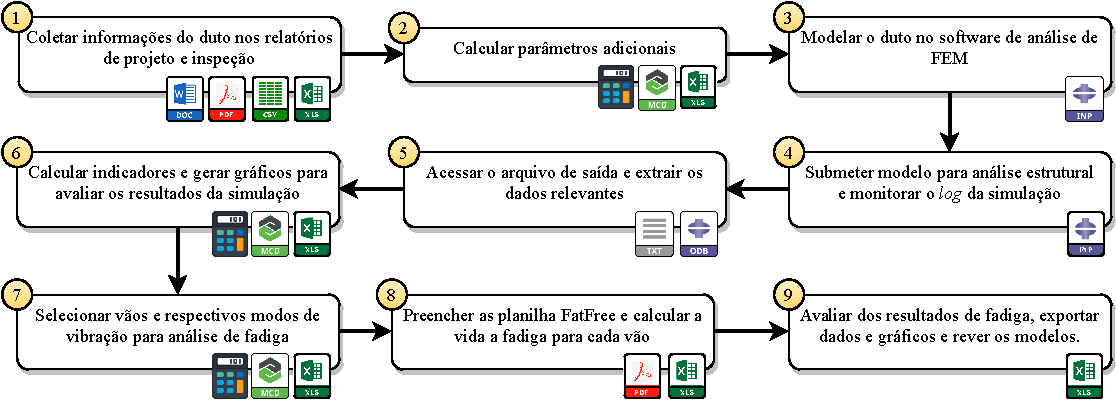
\includegraphics[width=\textwidth]{imagens/fluxograma.pdf}
    \fonte{Autor (2020)}
\end{figure}

A seguir, uma breve descrição de cada item:

\begin{enumerate}[label=(\arabic*)]
    \item Nesta etapa, o profissional reúne as informações básicas para construção dos modelos e outros dados usados em cálculos posteriores. Citadamente, temos aqui: os as cotas do perfil do duto e batimetria obtidas na inspeção, geometria e composição das camadas que compõem sessão do duto, parâmetros do solo, constantes físicas e coeficientes de segurança, posição e tipos de suportes ao longo do duto. Essa tarefa envole olhar uma série de documentos (\texttt{.doc}, \texttt{.pdf}, etc) em busca desses valores, dispostos de forma não estruturada. Quando estruturados, em forma de arquivos CSV ou planilhas, por exemplo, é necessário ainda manipular esses dados a fim de extrair somente a informação necessária ou convertê-las no formato apropriado. Um exemplo disso são os dados de batimetria, que precisam convertidos nas coordenadas dos nós de uma malha de elementos finitos no formato de um arquivo \texttt{.inp}. -- no caso do \abaqus.
    \item Uma vez de posse dos dados, e que nem todos os dados a serem utilizados estão de acordo com as especificações dos softwares a serem empregados na análise numéricas, ainda é necessários manipular alguns desses valores, seja calculando constantes ou convertendo unidades. Para isso, se pode-se utilizar softwares de planilhas e/ou folhas de cálculos (Microsft Excel, MathCad, Maple, etc.). Esta etapa inicia o pré-processamento dos dados.
    \item Com todos os dados em mãos, é necessário transformá-los em um modelo no software de elementos finitos, via interação com mouse e teclado, ou via arquivos de entrada. Embora a reutilização de arquivos de entrada previamente criados, nem todos os trechos desses arquivos são suficientes podem ser reaproveitados, especialmente trechos que precisam ser repetidos a depender da quantidade de certas entidades no modelo -- suportes, por exemplo. Esta etapa encerra o pré-processamento dos dados.
    \item Por mais simples que seja submeter o modelo para análise na maioria dos softwares de análise de elementos (alguns cliques via GUI\footnote{Graphical User Interface}, ou um comando via CLI\footnote{Command Line Interface}), as analises costumam levar horas, o que demanda o monitoramento do progresso da simulação a fim de realizar intervenções no modelo que não podem ser modeladas.  Esta etapa compreende a primeira parte do processamento propriamente dito.
    \item Uma vez concluída a simulação de elementos finitos, é necessário avaliá-los antes do pós-processamento. Extrair os resultados para as próximas análises. Dados que estes resultados estão armazenados em arquivos proprietários (como \texttt{.odb}, no caso do \abaqus) é necessário utilizar das ferramentas dos próprios pacotes de software de elementos finitos para isso. Esta tarefa, geralmente feita via GUI, costuma ser repetitiva e pode levar de alguns minutos ou horas. Esta etapa compreende a primeira parte do pós-processamento.
    \item De posse dos resultados em formatos acessíveis a outros software (MS Excel e MathCad, por exemplo), é necessário calcular (e muitas vezes visualizar em gráficos) alguns indicadores a fim de avaliar a validade dos resultados. Embora poderosos, estes softwares ainda carecem de gráficos mais interativos, como possibilidades de ampliar e transladar os gráficos com o mouse. Esta etapa inicia o pós-processamento.
    \item Para iniciar a análise de fadiga, é necessário escolher dentre os modos de vibração obtidos na simulação numérica aqueles que de fato tem influencia na fadiga. Para esta tarefa, existe a metodologia presente na \dnvf105 que
\end{enumerate}